\documentclass[a4paper]{article}

\usepackage{graphicx}
\usepackage[utf8]{inputenc}

%\usepackage[spanish]{babel}
\usepackage{geometry}


\usepackage{ntheorem,lipsum}

\theorembodyfont{\upshape}
\newtheorem{thm}{Teorema}[section]
\newtheorem{defi}{Definición}[section]
\newtheorem{obs}{Observación}[section]
\newtheorem{prop}{Proposition}[section]
\newtheorem{example}{Ejemplo}[section]
\newtheorem{problem}{Problem}[section]
\newtheorem{hipo}{Hipotesís}[section]

\usepackage{bm}

\usepackage{amsmath}
\usepackage{amssymb}


\title{Selective Harmonic Elimination via Optimal Control Theory}
\author{Jesús Oroya \\ Chair of Computational Mathematics}

\begin{document}

\maketitle

\begin{abstract}
    In this document, we study the selective harmonic elimination problem from view of point of a control theory. 
\end{abstract}
\tableofcontents
\newpage

\section{Introduction}

In this document, we propose  a optimal control  perspective of selective harmonic elimination problem (SHE) with symmetry of quarter wave and symmetry of half wave. 
%
In mathematical point of view, SHE problem can be seen as search of a square wave function  $f(\omega t ) \ | \ \omega t \in (0,2\pi)$ which have fixed a few Fourier coefficients. 
\newline

%
In this way, the $f(\omega t)$ can be written in Fourier series as follows:

\begin{gather}
    f(\omega t ) = \sum_{n=1}^\infty [a_n \cos(n\omega t) + b_n \sin(n \omega t)] 
\end{gather}

Where $a_n$ and $b_n$ coefficients are:
\begin{gather}
    a_n = \frac{1}{\pi} \int_0^{2\pi} f(\omega t ) \cos(n\omega t)d(\omega t) \label{an} \\
    b_n = \frac{1}{\pi} \int_0^{2\pi} f(\omega t ) \sin(n\omega t)d(\omega t) \label{bn}  
\end{gather}

\begin{problem}[SHE two levels]\label{SHEp}
    Given  $\bm{b}_T = [b^1_T \ , \ b^3_T \  , \ b^5_T \ , \ \dots \ , \ b^{N_b/2}_T] \in \mathbb{R}^{N/2}$ and  $\bm{a}_T = [a^1_T \ , \ a^3_T \  , \ a^5_T \ , \ \dots \ , \ a^{N_a/2}_T] \in \mathbb{R}^{N/2}$, we search a wave form $f(\omega t ) \ | \ \omega t \in (0,\pi/2)$ such that $f$ only can take values  $\{-1,1\}$ and its Fourier coefficients $b_n$ satisfies $b_n=b_T^n$ and  $a_n=a_T^n \ | \ \forall n \in \{1,3,\dots,N/2 \}$. 
\end{problem}

In the typical formulation of this problem, the function $f(\omega t)$ can be represented by locations  where the function $f(\omega t)$ changes its value, this locations are named switching angles.
%
Given a some vectors $\bm{a}^T$ and $\bm{b}^T$, the number of switching angles $M$ is \emph{a priori} unknown, so it's necessary fixed it. If we name switching angles as $\bm{\phi} = [\phi_1,\phi_2,\dots,\phi_M] \in \mathbb{R}^M $, we can simplify the Fourier coefficients as follows:

\begin{gather}
    a_n(\bm{\phi})  = \dots  \ | \ \forall n \ odd \\
    b_n(\bm{\phi})  =  \frac{4}{n\pi  } \bigg[ -1 + 2\sum_{i=1}^M  (-1)^{i+1}\cos(n\phi_i) \bigg] \ | \ \forall n \ odd
\end{gather}

With this expression, we can formulate the problem (\ref{SHEp}) as the next minimization problem:

\begin{problem}[Minimization problem for SHE]\label{SHEp_clas}
    \begin{gather}
        \min_{\bm{\phi} \in \mathbb{R}^m} \sum_{n \ odd}^{N/2}  \Bigg[ (a_n(\bm{\phi}) - a^n_T)^2 +  (b_n(\bm{\phi}) - b^n_T)^2  \Bigg]\\
        \text{subject to:} \begin{cases}
            0 < \phi_1  \\
            \phi_n < \phi_n+2 &  \forall n \in \{3,5,\dots,N/2-2 \}\\
            \phi_{N/2} < \pi/2
        \end{cases}
    \end{gather}     
\end{problem}

This formulation don't give a clearly procedure to choose a number of angles.
\newline

We propose consider a search of a function $f(\omega t)$ directly. In this way, instead of looking for the switching angles $\bm{\phi} \in \mathbb{R}^M$, we look for a function $f(\omega t) \in \{ g(\omega t)  \in L^\infty([0,\pi/2])\ /\ |g(\omega t)| < 1\} $. 

Thanks to fundamental calculus theorem, we can say:

\begin{gather}
    \alpha_n(\tau) = \frac{4}{\pi}\int_0^\tau f(\omega t) \sin(n\omega t)d(\omega t) 
    \Rightarrow
    \begin{cases} \label{ode}
        \frac{\partial \alpha_n}{d\tau} & = \frac{4}{\pi}f(\tau)\cos(n\tau) \\  
        \alpha_n(0) & = 0       
    \end{cases}
\end{gather}

\begin{gather}
    \beta_n(\tau) = \frac{4}{\pi}\int_0^\tau f(\omega t) \sin(n\omega t)d(\omega t) 
    \Rightarrow
    \begin{cases} \label{ode}
        \frac{\partial \beta}{d\tau} & = \frac{4}{\pi}f(\tau)\sin(n\tau) \\  
        \beta(0) & = 0       
    \end{cases}
\end{gather}


% Cuando resolvemos la ecuación diferencial ordinaria (\ref{ode}) hasta tiempo $T = \pi/2$ obtenemos el valor del coeficiente de Fourier $b_n$.

If we solve the ODE (\ref{ode}) from $\tau=0$ to $\tau=\pi/2$.
% Este se puede ver como una ecuación diferencial ordinaria controlada donde los estados del sistema son $\beta_n$ y el control es $f(\tau) \ | \ \tau \in [0,\pi/2]$.
%
So, this ODE can see as control system, where $\alpha_n(\tau)$ and $\beta_n(\tau) \ | \ \forall n $ is the states and $f(\tau)$ is the control variable.
%Entonces se puede plantear el problema de control cuyo objetivo es llevar el sistema $\beta_n(\tau)$ desde el estado nulo hasta $b_T^n$ para cada $n \in \{1,3,5,\dots,N/2 \}$ en un tiempo final $\tau_f = \pi/2$
In this way, the problem (\ref{SHEp}) can be solve via optimal control problem. 
\newpage
\part{Open Loop Optimal Control}

\section{Formulación del problema control óptimo}

Dado que el problema SHE es equivalente a controla un sistema dinámico desde el origen de coordenadas a un punto concreto, podemos formular el siguiente problema de control:
\begin{problem}[OCP para SHE en media onda]\label{OCP1}
    Dados dos conjuntos de números impares $\mathcal{E}_a$ and $\mathcal{E}_b$ con cardinalidades $|\mathcal{E}_a| = N_a$ y  $|\mathcal{E}_b| = N_b$ respectivamente, dados los vectores objetivos $\bm{a}_T  \in \mathbb{R}^{N_a}$ y $\bm{b}_T  \in \mathbb{R}^{N_b}$, buscamos la función  $f(\tau ) \ | \ \tau \in (0,\pi)$ que minimiza el siguiente funcional de coste:
        \begin{gather}
        J[f(\tau)] = \Bigg[ || \bm{a}_T - \bm{\alpha}(T)||^2 + || \bm{b}_T - \bm{\beta}(T)||^2 
        + \epsilon \int_0^{\pi} \mathcal{L}(f) d\tau \Bigg] 
    \end{gather}

    donde  $\bm{\alpha}(\tau) \in \mathbb{R}^{N_a} \times [0,\pi]$, $\bm{\beta}(\tau) \in \mathbb{R}^{N_b}  \times [0,\pi]$,  $||.||$ es la norma euclidea y $\epsilon$ es un parámetro pequeño que penaliza el funcional de coste con el término $\mathcal{L}(f):\mathbb{R} \rightarrow \mathbb{R}$. 
    \newline

    De esta forma podemos escribir el siguiente problema de control óptimo:
    \begin{gather}
        \min_{|f(\tau) |<1} J[f(\tau)] \\
        \notag \text{suject to: } \\
        \notag \forall i \in \mathcal{E}_a\ \ 
        \begin{cases}
            \dot{\alpha}_i(\tau) = (2/\pi) \cos(i\tau) f(\tau) & \tau \in [0,\pi]\label{dyn}\\
            \alpha_i(0) = 0
        \end{cases} \\
        \notag \forall j \in \mathcal{E}_b\ \ 
        \begin{cases}
            \dot{\beta}_j(\tau) = (2/\pi) \sin(j\tau) f(\tau) & \tau \in [0,\pi]\label{dyn}\\
            \beta_j(0) = 0
        \end{cases} 
    \end{gather}
\end{problem}

En el problema de SHE de dos niveles se busca una función $\{f(\tau) \ |  \tau \in [0,\pi] \}$  que solo pueda tomar los valores $\{-1,1\}$, sin embargo el problema (\ref{OCP1}) definido para un término de penelización $\mathcal{L}(f)$ arbitrario puede tomar valores en todo el intervalo $[-1,1]$. 
%
En teoría de control los controles que toma solo los valores extremos del intervalo son conocidos como controles \emph{bang-bang}. A continuación estudiaremos las condiciones que debe cumplir el término $\mathcal{L}(f)$ para que nuestro control óptimo sea una función escalón.

\subsection{Condiciones  para la obtención de controles \emph{bang-bang}}
A continuación estudiaremos las condiciones de optimilidad del problema con el fin de encontrar condiciones en el término $\mathcal{L}(f)$ que nos de el comportamiento \emph{bang-bang} en el control óptimo. 
%
Para ello utilizaremos el principio de máximo de Pontryagin \cite{pontryagin2018mathematical}, el cual formula varias condiciones de optimilidad para los problemas de control óptimo. 
%
Esta condiciones se formulan a través de un objeto llamado Hamiltoniano, que  en este caso se puede escribir como:


\begin{gather}\label{hamil}
    H(f,\bm{p}^\alpha(\tau),\bm{p}^\beta(\tau),\tau) = \epsilon \mathcal{L}(f) + 
    G(\bm{p}^\alpha(\tau),\bm{p}^\beta(\tau),\tau) f(\tau)
\end{gather}

Donde  hemos llamado $G(\bm{p}^\alpha,\bm{p}^\beta,\tau)$ a:
    \begin{gather}
        G(\bm{p}^\alpha,\bm{p}^\beta,\tau) = \frac{2}{\pi} \Bigg[ 
            \sum_{i \in \mathcal{E}_a} p^\alpha_i \cos(i\tau)+ 
            \sum_{j \in \mathcal{E}_b} p^\beta_j \sin(j\tau) 
        \Bigg]
    \end{gather}

y además donde hemos introducido las variables $\bm{p}^\alpha(\tau) \in \mathbb{R}^{N_a} \times [0,\pi]$ y $\bm{p}^\beta(\tau) \in \mathbb{R}^{N_b}  \times [0,\pi]$ son los estados adjuntos correspondientes a los estados $\bm{\alpha}$ y $\bm{\beta}$ respectivamente.  
%
Aunque el valor exacto de los coestados es necesario para obtener el control óptimo, las condiciones necesarias para obtener controles \emph{bang-bang} son independientes del valor de estos. Por esta razón, suponemos que el valor de los coestados óptimos $\bm{p}_*^\alpha$ y $\bm{p}_*^\beta$ son conocidos.
\newline 

Por otra parte, utilizando otra condición del principio del máximo:
\begin{gather}
    H(\tau,\bm{p}_*^\alpha,\bm{p}^\beta_*,f_*) \leq H(\tau,\bm{p}_*^\alpha,\bm{p}^\beta_*,f)
\end{gather}
podemos obtener la forma del control óptimo cuando los co-estados óptimos $\bm{p}_*^\alpha$ y $\bm{p}_*^\beta$ además de la variable temporal $\tau$ están fijas. 
%
Entonces el problema se reduce la minimización de una función $H^*(f) = H(\tau,\bm{p}_*^\alpha,\bm{p}^\beta_*,f)$ en una variable $f$ dentro del intervalo $[-1,1]$.
%
Dado que necesitamos que el control óptimo $f^*$ sea \emph{bang-bang}, debemos diseñar  $H^*(f)$ de manera que su mímino esté en los extremos del intervalo $[-1,1]$.
%
En el caso de una variable (este caso) solo podemos conseguir este comportamiento si no existe ningún mínimo dentro del intervalo. Una manera de asegurar este comportamiento es tomando la función $H^*(f)$ concava, mediante la elección el término $\mathcal{L}(f)$. 
%
Eso se debe a que la concavidad de el término $\mathcal{L}(f)$ determina la concavidad del Hamiltoniano $H^*(f)$ gracias a que la derivada segunda de $H^*(f)$ es proporcional al la derivada segunda del término de penalización, es decir:
\begin{gather}
    \frac{d^2{H^*}^2}{df^2} = \epsilon \frac{d^2\mathcal{L}(f)}{df^2} 
\end{gather}

De esta manera siempre que elijamos un término de penalización tal que:

\begin{gather}
    \frac{d^2L[f]}{df^2} \leq 0 
\end{gather}

obtendremos un función $H^*(f)$ cóncava dentro de un intervalo convexo dando lugar a un control óptimo $f^*$  \emph{bang-bang}. Podemos ver una ilustración de este comportamiento en la figura (\ref{bang-bang}).
\newline

\begin{figure}[!ht]
    \centering
    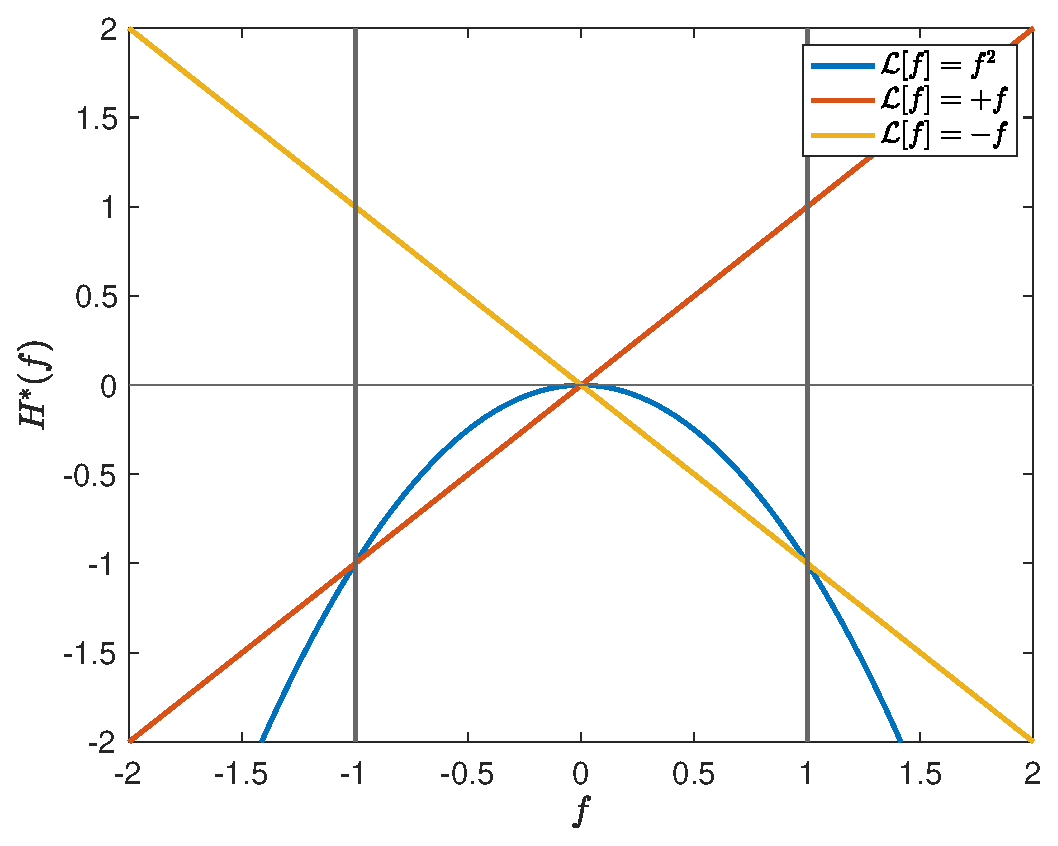
\includegraphics[scale=0.5]{img/bang-bang.eps}
    \caption{Ilustración sobre el comportamiento de la función $H^*(f)$ para distintos términos de penalización $\mathcal{L}(f)$. El problema de minimización de $H^*(f)$ con respecto a $f$ para las distintas curvas presentadas en la figura siempre tiene minimos en los extremos del intervalo $[-1,1]$ de manera que el control óptimo en los tres casos, será \emph{bang-bang}.}
    \label{bang-bang}
\end{figure}


\subsection{OC SHE de dos niveles con simetría de cuarto de onda} 

Consideraremos un caso concreto del problema presentado en la sección anterior. Este es problema de SHE con simetría de cuarto de onda, es decir consideramos que la función $f(\tau)$ cumple la siguiente expresión:
\begin{gather}
    f(\tau + \pi/2)   = f(\tau)    \ | \ \tau \in (0,\pi/2)
\end{gather}

Esta expresión nos permite simplificar la expresión para los coeficientes de Fourier (\ref{an}) and (\ref{bn}) de la siguiente manera:
\begin{align}
    a_i = & \  0 \ \ | \  \ \forall i \in \mathbb{Z} \\
    b_j = &  \frac{4}{\pi} \int_0^{\pi/2} f(\tau ) \sin(j\tau)d\tau \ | \ \forall j \ odd
\end{align}

Entonces  $f(\tau) \ | \ \tau \in (0,\pi/2)$ puede ser escrita como:
\begin{gather}
    f(\tau ) = \sum_{j \ odd}^\infty  b_j \sin(j \tau) \\
    b_j = \frac{4}{\pi}\int_0^{\pi/2} f(\tau ) \sin(j\tau)d\tau \ \ | \ \ j \ odd \label{bn_odd}
\end{gather}

En este contexto podemos definir el siguiente problema de control de manera análoga que en la subsección anterior:
\begin{problem}[OCP para SHE en cuarto de onda]\label{OCP_bn}
    Dado un conjunto de número impares $\mathcal{E}_b$ con cardinalidad $|\mathcal{E}_b| = N_b$ y dado un vector objetivo $\bm{b}_T  \in \mathbb{R}^{N_b}$, buscamos la función $f(\tau ) \ | \ \tau \in (0,\pi/2)$ tal que  $f(\tau)$ minimize el siguiente funcional de coste:

        \begin{gather}
        J[f(\tau)] = \Bigg[ || \bm{b}_T - \bm{\beta}(T)||^2 + \epsilon \int_0^{\pi/2} \mathcal{L}(f(\tau)) d\tau \Bigg] 
    \end{gather}

    donde $ \bm{\beta}(\tau) \in \mathbb{R}^{N_b} \times [0,\pi/2] $,  $||.||$ es la norma euclidea y $\epsilon$ es un parámetro de penalización para el término $\mathcal{L}(f)$.
    \newline

    Entonces el problema de control se puede escribir como:
    \begin{gather}
        \min_{|f(\tau) |<1} J[f(\tau)] \\
        \notag \text{suject to: } \\
        \notag \forall j \in \mathcal{E}_b \
        \begin{cases}
            \dot{\beta_j}(\tau) = (4/\pi) \sin(j\tau) f(\tau) & \tau \in [0,\pi/2]\label{dyn}\\
            \beta_j(0) = 0
        \end{cases} 
    \end{gather}
\end{problem}

En este caso el problema de control tiene el siguiente Hamiltoniano:
\begin{gather}
    H(f,\bm{p}_\beta,\tau) = \epsilon  \mathcal{L}(f)+ 
    \frac{4f}{\pi} \Bigg[ 
        \sum_{j \in \mathcal{E}_b} p^\beta_j \sin(j\tau) 
    \Bigg]
\end{gather}

Podemos ver que el Hamiltoniano tiene la misma estructura que (\ref{hamil}), por lo que de la misma forma la elección de un término de penalización $\mathcal{L}(f)$ concavo nos produce un Hamiltoniano $H^*(f)$ cóncavo y por tanto un control óptimo $f^*$ \emph{bang-bang}.

\section{Numerical experiments}

To solve the optimal control problem, we use a direct method. %
%
This method considered a time discretization. In this way, if we have a partition $\{\tau_0,\tau_1,\dots,\tau_{N_t}\}$ of interval $[0,\pi/2]$ , we can represent a function $\{ f(\tau) \ | \ \tau \in [0,\pi/2]\}$ as a vector $\bm{f} \in \mathbb{R}^{N_t}$ where component $f_i = f(t_i)$. Then the optimal control problem (\ref{SHEp}) can be written as optimization problem with variable $\bm{f} \in \mathbb{R}^{N_t}$.

\begin{problem}
    Given  $\bm{b}_T  \in \mathbb{R}^{n_b}$,  the optimization problem can be write: 
    \begin{gather}
        \min_{\bm{f} \in \mathbb{R}^{N_t} } \Bigg[ || \bm{b}_T - \bm{\beta}^{N_t}||^2 - \epsilon \Delta\tau  \sum_{i=0}^{N_t} f_{\tau_i}^2 \Bigg]  \\
        \text{suject to: }
        \begin{cases}
            \beta_n^{i+1} = \beta_n^{i} + \Delta \tau (4/\pi) \sin(n\tau_i) f_\tau & \tau \in [0,\pi/2]\label{dyn}\\
            \beta_n^0 = 0
        \end{cases} \\
        \notag \forall n \in \{1,3,5,\dots,N/2 \}
    \end{gather}
\end{problem}

Where we use a euler scheme to discretizate the dynamics. This problem is a Nonlinear programming, for this we use CasADi software to solve.

\subsection{Numerical result for SHE of two levels}

We considered the harmonics $[\beta_1,\beta_5,\beta_7,\beta_{11}]$. We want waveform that  $\bm{b}_T = [b_T^1,b_T^5,b_T^7,b_T^{11}] = [m_a,0,0,0,0]$, where $m_a$ is a parameter . We will compare the different solutions of problem (\ref{SHEp_clas}).
Compararemos el problema mediante soluciones obtenidas del problema (\ref{SHEp_clas}), mediante algoritmos genéticos.

El problema de control óptimo (\ref{OCP1}) reproduce una de las soluciones obtenidas 

\begin{figure}
        \centering
        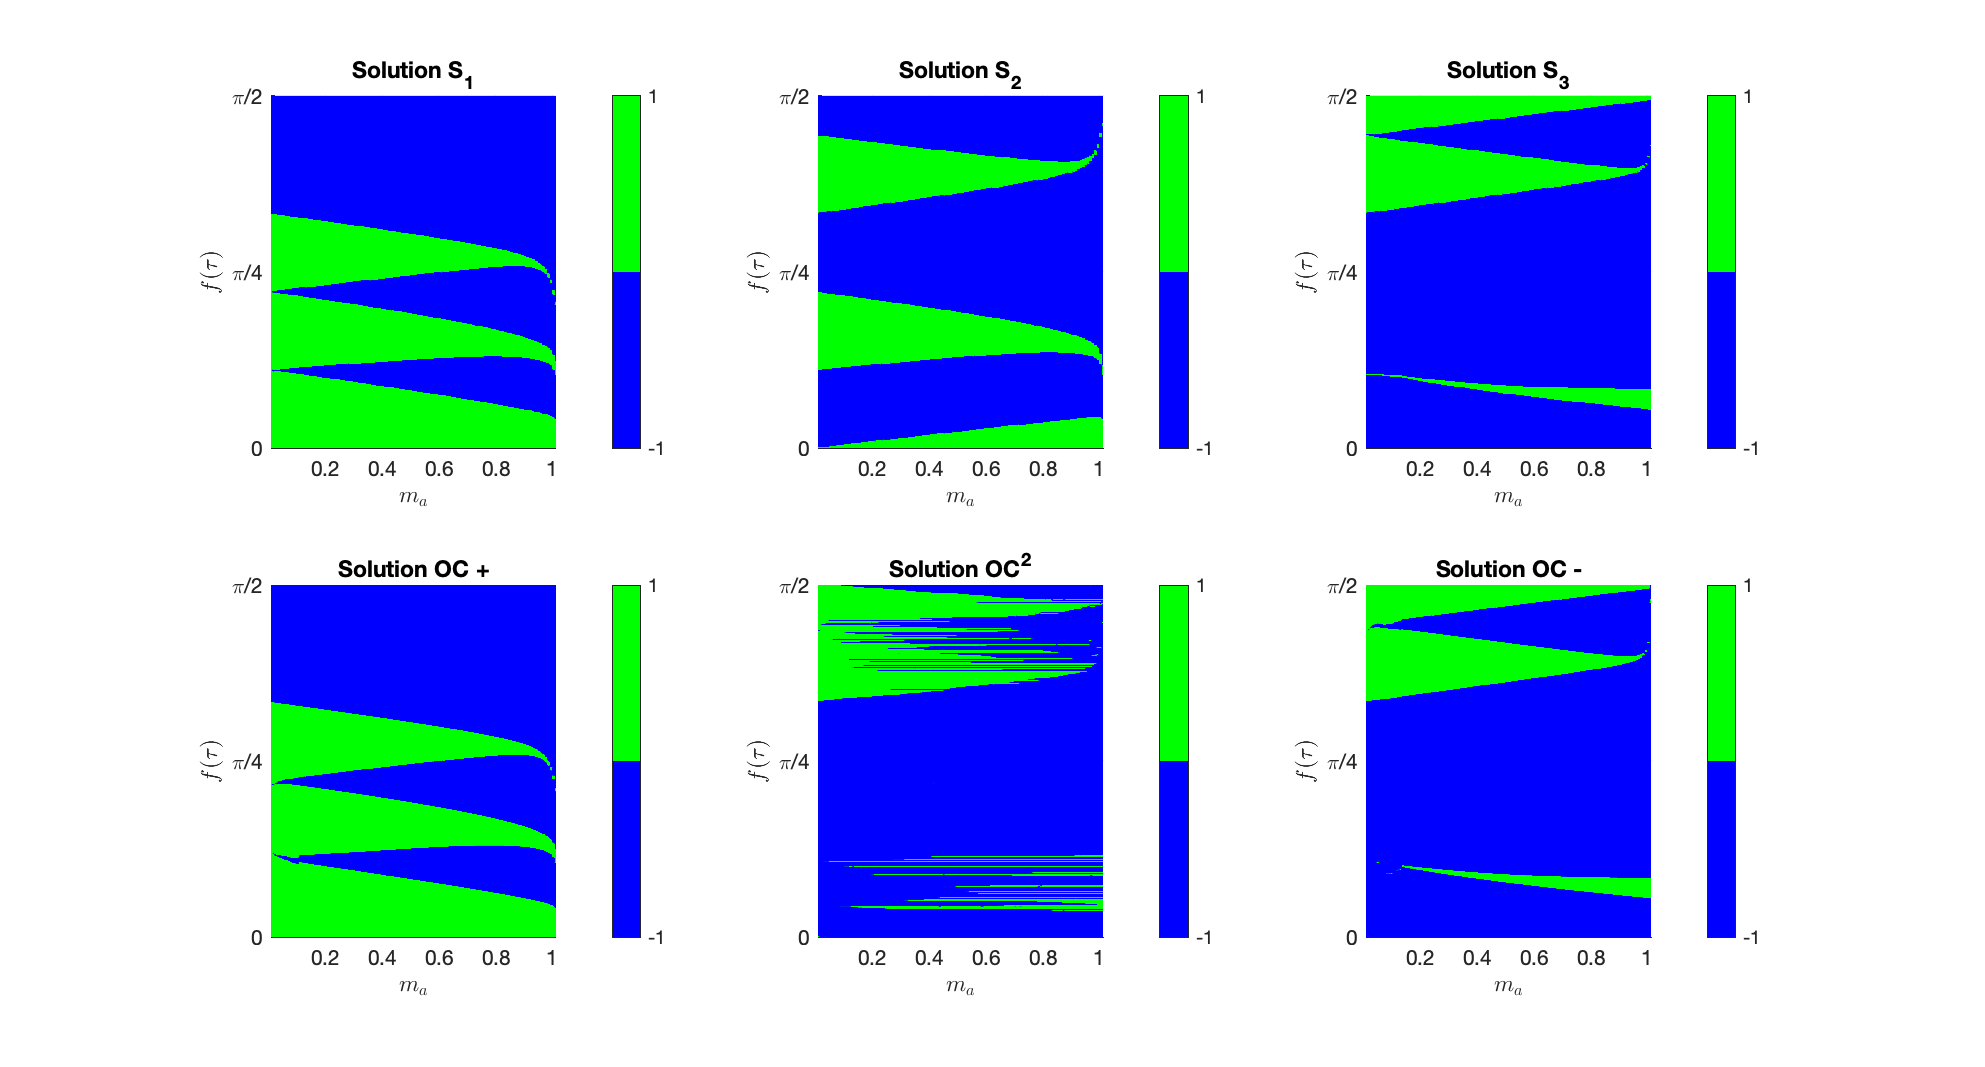
\includegraphics[scale=0.35]{img/EX01_surf.eps}
        \caption{Comparison of solutions for different values of $m_a$. Solutions $S_1$, $S_2$, $S_3$ correspond to problem (\ref{SHEp_clas}) where the number of switching angles is prefixed, while $OC$ solution correspond to optimal control problem.}
        \label{fig:solutions}
    \end{figure}



\begin{figure}
    \centering
    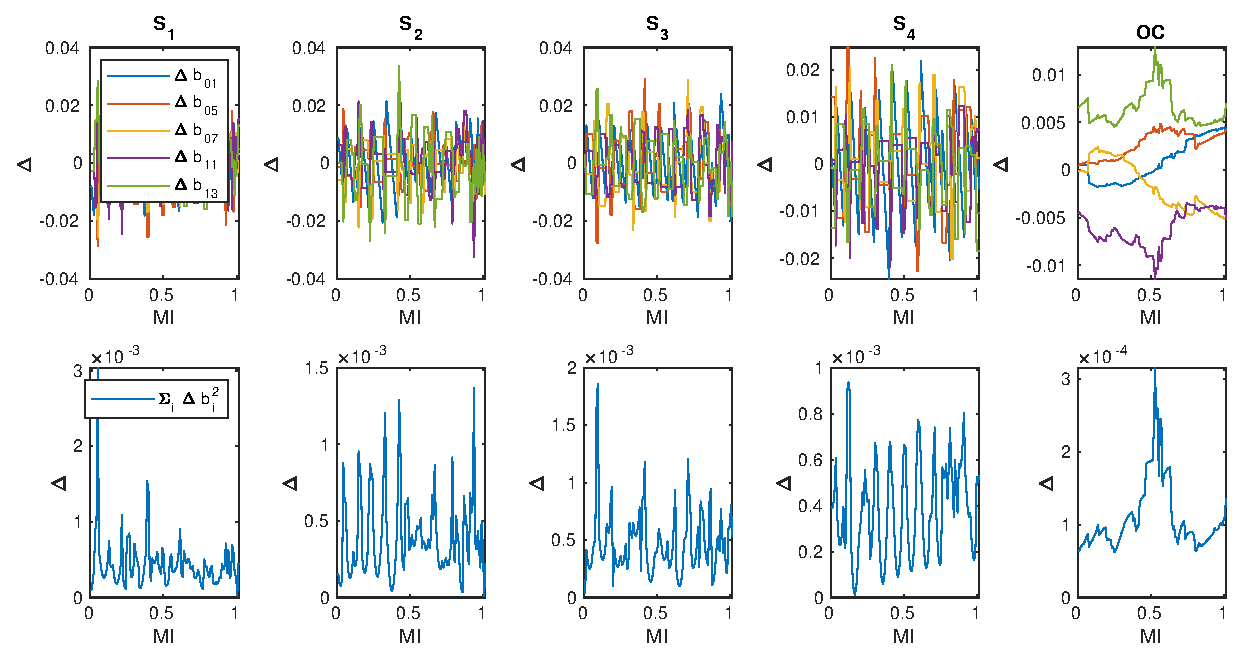
\includegraphics[scale=0.7]{img/EX01.eps}
    \caption{The order of magnitud of the square of euclidean distantes to target is the same for all solutions of figure (\ref{fig:solutions})}
\end{figure}

\subsection{Numerical result for SHE of three levels}

%%%%%%%%%%%%%%%%%%%%%%%%%%%%%%%%%%%%%%%%%%%%%%%%%%%%%%%%%%%

\begin{figure}
    \centering
    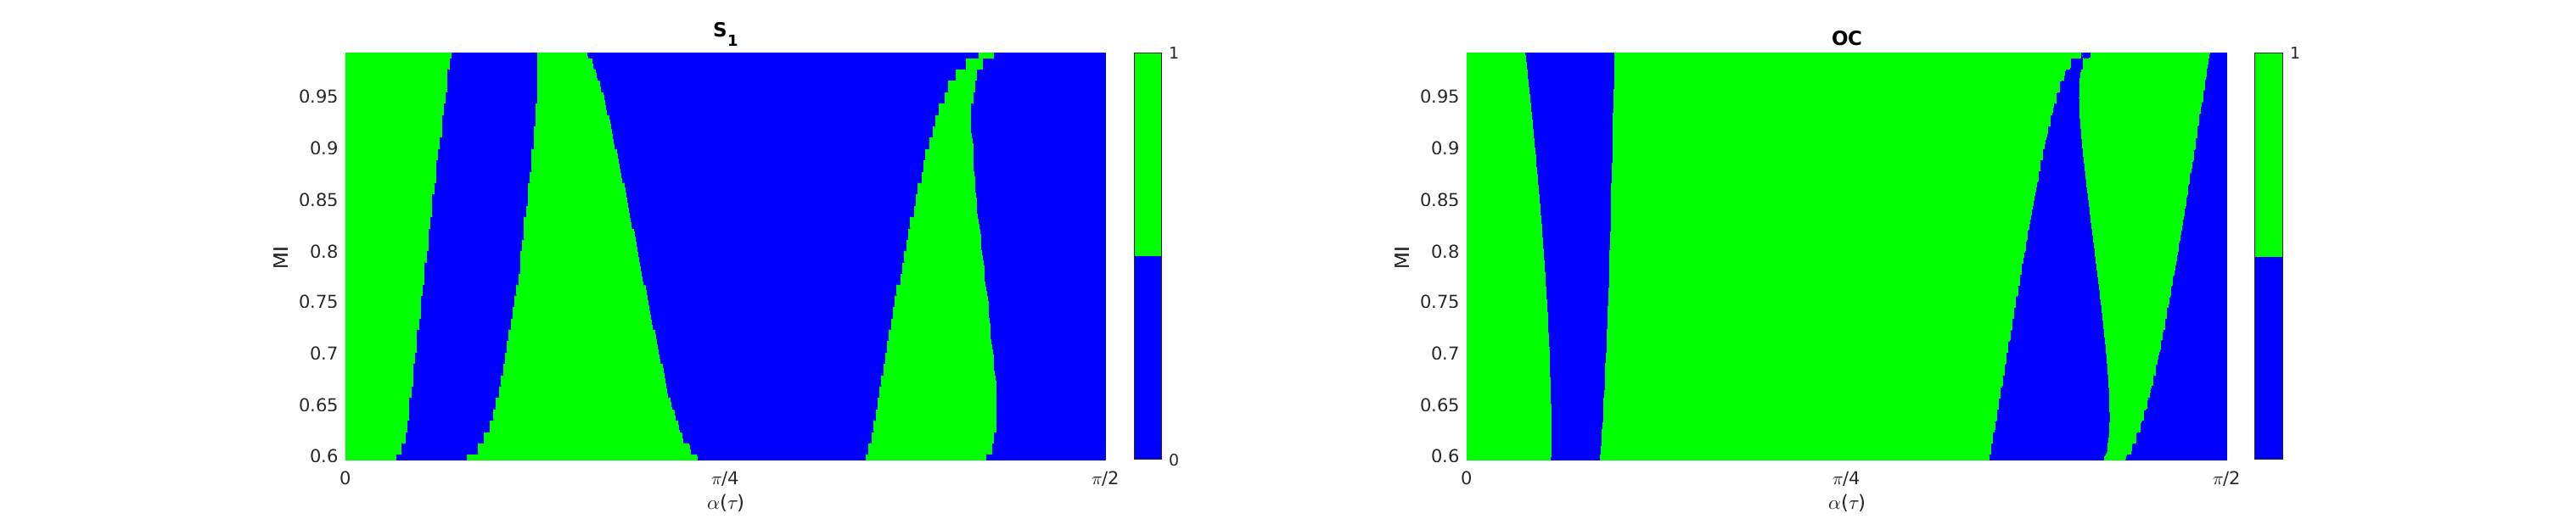
\includegraphics[scale=0.35]{img/EX01_surf_3LVL.eps}
    \caption{Solutions}
\end{figure}



\begin{figure}
    \centering
    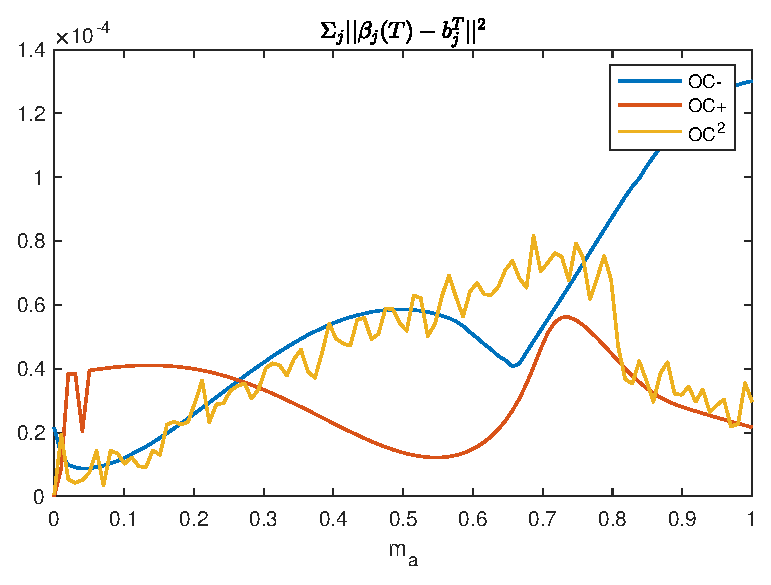
\includegraphics[scale=0.6]{img/EX01_3LVL.eps}
    \caption{Errors}
\end{figure}


\newpage
\part{Feedback Optimal Control}
\section{SHE two levels with quarter-wave symmetry as dynamic programming problem}

Con el fin de encontrar la solución al problema para distintos targets $\bm{a}_T$ y $\bm{b}_T$ consideraremos el cambio de variable $\bm{\beta}'(\tau) = \bm{\beta}(\tau) - \bm{b}_T$. De manera que, podemos plantear un problema de control donde el estado inicial el target $\bm{b}_T$ y cuyo objetivo es llevar el sistema al origen de coordenadas.
\begin{problem}
    Given  $\bm{b}_T  \in \mathbb{R}^{n_b}$, we define a cost functional in this way: 
        \begin{gather}
        J[f(\tau)] =  \frac{1}{2}|| \bm{\beta}(T)||^2  
    \end{gather}


    So, the optimization problem can be write: 
    \begin{gather}
        \min_{f \in \{-1,1\} } J[f(\tau)]) \\
        \text{suject to: }
        \begin{cases}
            \frac{d\beta_n(\tau)}{d\tau} =  - (4/\pi) \sin(n\tau) f(\tau) & \tau \in [0,\pi/2]\label{dyn}\\
            \beta_n(0) = b_T^n
        \end{cases} \\
        \notag \forall n \in \{1,3,5,\dots,N_b/2 \}
    \end{gather}
    
\end{problem}

Tomamo un discretización $\{\tau_0,\tau_1,\dots,\tau_{N_t} \}$ del intervalo $[0,\pi/2]$. Entonces podemos discretizar el problema anterior:

\begin{problem}
    Given  $\bm{b}_T  \in \mathbb{R}^{n_b}$,  the optimization problem can be write: 
    \begin{gather}
        \min_{\bm{f} \in \mathbb{R}^{N_t} } \frac{1}{2}||\bm{\beta}^{N_t}||^2 \\
        \text{suject to: }
        \begin{cases}
            \beta_n^{i+1} = \beta_n^{i} - \Delta \tau (4/\pi) \sin(n\tau_i) f_\tau & \tau \in [0,\pi/2]\label{dyn}\\
            \beta_n^0 = b_T^n
        \end{cases} \\
        \notag \forall n \in \{1,3,5,\dots,N/2 \}
    \end{gather}

\end{problem}

\subsection{Dynamic programming}

Función valor 

\begin{gather}
    v_t(\bm{b}_T) =  \min_{\bm{f} \in \mathbb{R}^{N_t-t} } \frac{1}{2}||\bm{\beta}^{t}||^2 \\
    \text{suject to: }
    \begin{cases}
        \beta_n^{i+1} = \beta_n^{i} - \Delta \tau (4/\pi) \sin(n\tau_i) f_\tau & \tau \in [0,\pi/2]\label{dyn}\\
        \beta_n^0 = b_T^n
    \end{cases} \\
    \notag \forall n \in \{1,3,5,\dots,N/2 \}
\end{gather}




Entonces la función valor de estado cumple la ecuación de Bellman, que en este caso se puede escribir como:
\begin{gather}\label{BellmanEquationOptimo}
    v_t(\bm{\beta}^t) = \min_{f \in \{ -1,1 \}}  v_{t+1}(\bm{\beta}^{t+1})  \\
    v^{N_t}(\bm{\beta}^{N_t}) =  \frac{1}{2}|| \bm{\beta}^{N_t}||^2
\end{gather}

La función $v_t(\bm{\beta}^t)$ representa el mejor coste que se puede alcanzar desde el estado $\bm{\beta}^t$ en $(N_t-t)$ pasos. Es por ello que en $t=Nt$ el mejor coste que se puede alcanzar desde el punto $\bm{\beta}^t$ es el valor del coste final $\frac{1}{2} || \bm{\beta}^{N_t}||^2$


Luego el control óptimo se puede calcular mediante la siguiente expresión 

\begin{gather}
    f^*(\tau,\bm{\beta}_t) = \min_{f \in \{ -1,1\}} v_t(\bm{\beta}_t)
\end{gather}

% \begin{algorithm}[!ht]
%     \caption{\emph{Value Iteration}}\label{ValueIteration}
%     \begin{algorithmic}[1]
%         \Procedure{Value-Iteration}{$\mathcal{V}^*,tol$}
%         \State $k \gets 0$
%         \State $\mathcal{V}_k\gets \mathcal{V}^*$
%         \While{$error\leq tol$}
%             \State $k \gets k + 1$
%             \For{$\forall s \in \Ss$}
%                 \State $\mathcal{V}_k(s)\gets \mathcal{T}_v\mathcal{V}_{k-1}(s)$
%             \EndFor
%             \State $error \gets || \mathcal{V}_k - \mathcal{V}_{k-1}||_\infty$
%         \EndWhile
%         \State $\displaystyle \pi_k^*(s) = \arg \max_{a'\in \As} \bigg[ r(s,a') + \gamma \sum_{s'}p(s'|s,a') v_*(s')
%         \bigg]$
%         \State \textbf{return}: [$\mathcal{V}_k(s)$,$\pi_k^*(s)$]
%         \EndProcedure
%     \end{algorithmic}
% \end{algorithm}

\newpage
\appendix


\section{Other}


\begin{gather}
    \int_0^{\pi/2} ||f(\tau) ||^2 d\tau = \pi/2
\end{gather}

\begin{gather}
    \int_0^{\pi/2} ||f(\tau) ||^2 d\tau = \pi/2
    \int_0^{\pi/2} || \sum_{n \ odd}^\infty b_n \sin(n\tau) ||^2 d\tau = \pi/2\\
    \int_0^{\pi/2}  \sum_{n,n' \ odd}^\infty b_n b_n' \sin(n\tau)\sin(n'\tau)  d\tau = \pi/2\\
    \sum_{n,n' \ odd}^\infty b_n b_n' \int_0^{\pi/2}\sin(n\tau)\sin(n'\tau)  d\tau = \pi/2 \\
    ?? \\
    \frac{\pi}{4} \sum_{n \ odd}^\infty b_n^2  = \pi/2 \\
    \sum_{n \ odd}^\infty b_n^2  = 2 
\end{gather}

 
\bibliographystyle{apalike}
\bibliography{bib}

\end{document}